\usetikzlibrary{decorations.markings,calc}
\begin{activity}{Boundary Conditions and Geological Meaning}

\section*{Purpose}
To understand how boundary conditions encode geological assumptions in numerical
models.

A numerical model does not ``know'' geology—it only knows equations and boundary
conditions.

{\color{red}
\section*{Learning Outcomes}

By the end of this activity, you should be able to:
\begin{itemize}
    \item Distinguish between Dirichlet (fixed value) and Neumann (fixed flux) boundary conditions.
    \item Match appropriate boundary conditions to geological settings (ocean floor, continental lithosphere, cooling intrusion).
    \item Explain how changing a boundary condition changes the physical system the model represents.
    \item Argue why inappropriate boundary conditions can produce physically misleading results even when the numerical solution is mathematically stable.
\end{itemize}
}

\emph{Boundary conditions determine what kind of Earth your model represents.}

\ntextbox{Boundary Conditions}{
    A PDE describes how a field behaves \emph{inside} a domain, $\Omega$. To get a unique solution we must also specify how the domain interacts with its surroundings along the boundary, $\partial\Omega$. That extra information is the \textbf{boundary condition} and geologically, it is where an assumption about the outside world enters the model.
    \begin{center}
    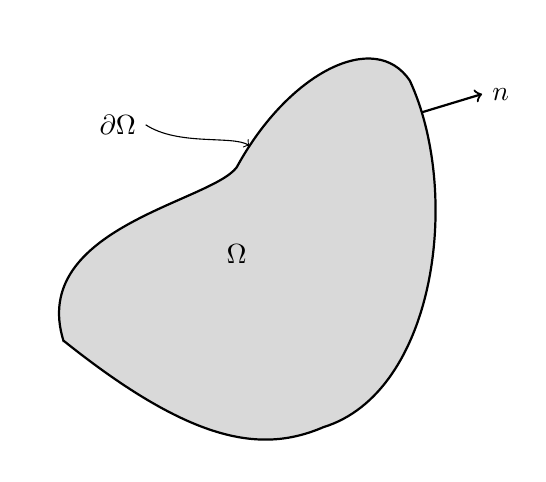
\begin{tikzpicture}[scale=1.1]
        \newcommand{\curve}{
            (-2,-1)
            .. controls (-0.5,-2.2) and (0.3,-2.3) ..
            (1,-2)
            .. controls (2.3,-1.6) and (2.6,0.7) ..
            (2,2)
            .. controls (1.6,2.6) and (0.6,2.1) ..
            (0,1)
            .. controls (-0.3,0.6) and (-2.4,0.3) ..
            cycle;
        }

        \draw[
            thick,
            fill=gray!30,
            postaction={
            decorate,
            decoration={
                markings,
                mark=at position 0.55 with {
                \draw[->,thick] (0,0) -- (0,-0.8);
                \node[right] at (0,-0.8) {$\vu n$};
                },
                mark=at position 0.75 with {
                \draw[<-,thin] (0,0) .. controls (0,-0.25) and (0.5,-0.75) .. (0.5,-1.25) node[left] {$\partial\Omega$};
                }
            }
        }
        ] \curve;

    \node at (0,0) {$\Omega$};
    \end{tikzpicture}
    \end{center}

    For a field $u(\vb{x})$, four standard conditions prescribe different combinations of the boundary value $u$ and normal flux $\pdv{u}{\vu{n}}$ on $\partial\Omega$, with the first two types being most common and the second two being special cases:

    \begin{center}
    Types of boundary conditions applied to domain boundaries.
    \begin{tabularx}{\textwidth}{@{}lXcX@{}}
        \toprule
        \textbf{Type} & \textbf{Physical meaning} & \textbf{Prescribes on $\partial\Omega$} & \textbf{Example} \\
        \midrule
        \textbf{Dirichlet} &
        environment imposes fixed value at $\partial\Omega$ &
        $u = f(\vb{x})$ (Type I)&
        Ocean floor: $T_\text{surf} = \SI{4}{^\circ C}$ \\
        \textbf{Neumann} &
        environment imposes fixed rate of energy, mass, current, etc.\ transfer across $\partial\Omega$ &
        $\displaystyle{\pdv{u}{\vu{n}}} = g(\mathbf{x})$ (Type II) &
        Mantle heat flux entering the base of the lithosphere \\
        \textbf{Robin} &
        process links value \& flux at $\partial\Omega$ &
        $au + b \displaystyle{\pdv{u}{\vu{n}}} = c$ &
        Intrusion cooling by exchange with country rock:
        $-k\,\partial T/\partial n = h(T-T_\text{melt})$ \\
        \textbf{Cauchy} &
        $\partial\Omega$ strongly constrained by independent observations &
        $u = f(\vu{x}),\ \displaystyle{\pdv{u}{\vu{n}}}=g(\mathbf{x})$ &
        Borehole where both $T$ and heat flow are measured \\
        \bottomrule
    \end{tabularx}
    \end{center}

    The governing equation describes the physics \emph{inside} the domain; boundary conditions describe how the model interacts with the outside world.  Two models with the same PDE and physical properties can produce completely different results if different boundary conditions are chosen — choosing a boundary condition is a geological modelling decision, not merely a mathematical one.
}{core}



% Dirichlet Examples:
% \begin{itemize}
% \item Fixed ocean-bottom temperature.
% \item Fixed atmospheric temperature at Earth's surface.
% \item Fixed hydraulic head in a groundwater model.
% \item Fixed gravitational potential on a far-field boundary.
% \end{itemize}


% Neumann Examples:
% \begin{itemize}
% \item Mantle heat flux entering the base of the lithosphere.
% \item Groundwater recharge entering an aquifer.
% \item Prescribed electrical current density in an electrical model.
% \end{itemize}

% Robin Examples:
% \begin{itemize}
% \item Heat exchange between rock and the atmosphere.
% \item Cooling of a magmatic intrusion by surrounding country rock.
% \item Groundwater leakage through a semi-permeable boundary.
% \end{itemize}

% Cauchy Examples:
% \begin{itemize}
% \item A borehole where both temperature and heat flow are measured.
% \item A boundary constrained simultaneously by observed hydraulic head and groundwater flux.
% \item Inverse problems where multiple independent observations are available along a boundary.
% \end{itemize}

\begin{questions}
    \question{Thermal evolution scenarios}
    Boundary conditions matter for evolving systems too, not just steady ones.

    For each, state which boundary condition type you would use at the boundary relevant to its thermal evolution, and justify your choice physically.

    \begin{center}
        \begin{tblr}{
            colspec={lllX},
            hline{3-Z} = {dashed},
            hline{1,2,Z} = {solid},
            vline{1,2,5} = {solid},
            vline{3-4} = {dashed},
            row{1} = {font=\bfseries},
            row{2-Z} = {ht=2.5em},
        }
            Case & Upper BC & Lower BC & Why? \\
            sedimentation/erosion & & & \\
            cooling pluton & & & \\
            hotspot & & & \\
            cooling oceanic plate & & & \\
            stable continental lithosphere & & & \\
        \end{tblr}
    \end{center}

    \question{What the borehole tells you}
    The oceanic case fits the seafloor to a single condition: seawater keeps the seafloor close to a fixed temperature (Dirichlet). Continental lithosphere is different; a borehole gives you both a temperature and a gradient (hence heat flow) at the same location.

    \textbf{Which boundary condition type does that make?} Referring back to the summary table, explain why the continental case cannot be reduced to a single fixed value or a single fixed flux the way the oceanic case can.

    Heat flow is also measured at the seafloor, away from zones of active hydrothermal circulation, and is used to test age-dependent cooling models through time---\emph{even though it is not imposed as a boundary condition there}. \textbf{Why is oceanic heat flow used to test the model rather than to set its boundary condition?}
    \answerbox[4cm]

    \question{Extension --- the lower boundary}
    \textit{This question is more open-ended than the others --- there isn't a single clean answer, and that's the point.}

    For continental lithosphere, the base is often assigned a fixed temperature at the mantle adiabat. But unlike a borehole measurement, we don't know in advance how deep that boundary should sit.

    If heat production $A(z)$ is specified through the crust, conservation of energy links the heat flow entering the base, $q_b$, to the heat flow measured at the surface, $q_0$:
    \[
        q_0 = q_b + \int_0^{z_b} A(z)\,\dd z
    \]
    where $z_b$ is the depth of the lower boundary.

    \textbf{Explain} why fixing $T$ to the mantle adiabat at the base makes this a harder problem than fixing $T$ at a known depth. What quantity has to be solved for, rather than simply assumed?
    \answerbox[4cm]

    \question{Critical thinking}
    \textbf{Task:}
    Explain why inappropriate boundary conditions can produce physically misleading results—even if the numerical solution is mathematically stable.
    \answerbox[3cm]

    \textbf{Reflection} \\
    If two models use the same equation but different boundary conditions, can they produce completely different results? Why?
    \answerbox[3cm]
\end{questions}

\bigskip

\section*{Key Ideas}

Boundary conditions are where geological assumptions enter a numerical model.

\textbf{Boundary conditions define the physical system, not just the mathematics.} Two models with identical equations but different boundary conditions represent completely different geological systems. Choosing a fixed temperature surface is equivalent to assuming an ocean floor in contact with circulating seawater; choosing a fixed heat flux is equivalent to assuming a continental surface where temperatures are free to evolve.

\textbf{Dirichlet and Neumann conditions represent different physical constraints.} A Dirichlet condition fixes the value (e.g., temperature); a Neumann condition fixes the gradient (e.g., heat flow across the surface). Robin and Cauchy boundary conditions are combinations of Dirichlet and Neumann conditions, either in linked or independent, respectively.

\begin{figure}[h]
\centering
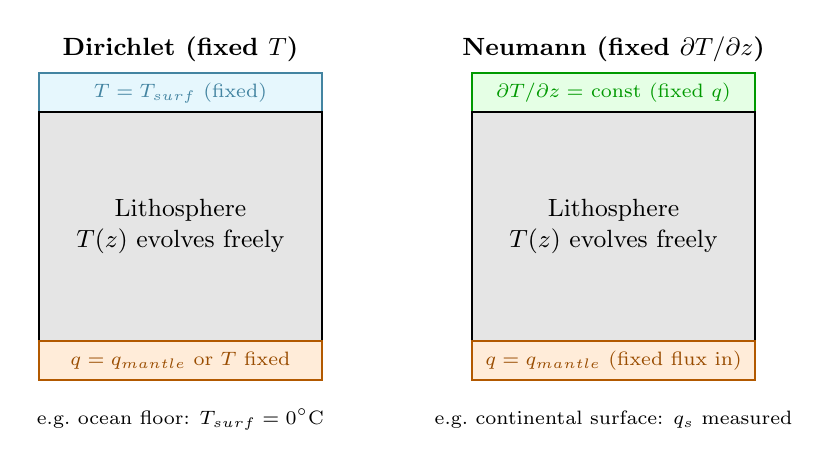
\begin{tikzpicture}[scale=1.0,
  box/.style={draw, thick, fill=blue!8, minimum width=3.5cm, minimum height=1.0cm, align=center, font=\small},
  bcbox/.style={draw, thick, rounded corners, minimum width=3.2cm, minimum height=0.8cm, align=center, font=\scriptsize},
  arr/.style={->, thick}
]
  % --- Dirichlet ---
  \node[font=\small\bfseries] at (2.0, 4.2) {Dirichlet (fixed $T$)};
  \draw[fill=cyan!10, draw=cyan!60!black, thick] (0.2, 3.4) rectangle (3.8, 3.9);
  \node[font=\scriptsize, cyan!60!black] at (2.0, 3.65) {$T = T_\text{surf}$ (fixed)};
  \draw[fill=gray!20, thick] (0.2, 0.5) rectangle (3.8, 3.4);
  \node[font=\small, align=center] at (2.0, 1.95) {Lithosphere\\$T(z)$ evolves freely};
  \draw[fill=orange!15, draw=orange!70!black, thick] (0.2, 0.0) rectangle (3.8, 0.5);
  \node[font=\scriptsize, orange!60!black] at (2.0, 0.25) {$q = q_\text{mantle}$ or $T$ fixed};
  \node[font=\scriptsize, align=left] at (2.0,-0.5) {e.g.\ ocean floor: $T_\text{surf} = 0^\circ$C};

  % --- Neumann ---
  \node[font=\small\bfseries] at (7.5, 4.2) {Neumann (fixed $\partial T/\partial z$)};
  \draw[fill=green!10, draw=green!60!black, thick] (5.7, 3.4) rectangle (9.3, 3.9);
  \node[font=\scriptsize, green!60!black] at (7.5, 3.65) {$\partial T/\partial z = $ const (fixed $q$)};
  \draw[fill=gray!20, thick] (5.7, 0.5) rectangle (9.3, 3.4);
  \node[font=\small, align=center] at (7.5, 1.95) {Lithosphere\\$T(z)$ evolves freely};
  \draw[fill=orange!15, draw=orange!70!black, thick] (5.7, 0.0) rectangle (9.3, 0.5);
  \node[font=\scriptsize, orange!60!black] at (7.5, 0.25) {$q = q_\text{mantle}$ (fixed flux in)};
  \node[font=\scriptsize, align=left] at (7.5,-0.5) {e.g.\ continental surface: $q_s$ measured};
\end{tikzpicture}
\caption{Dirichlet (left) fixes temperature at a boundary — appropriate where temperature is controlled externally (ocean floor). Neumann (right) fixes the heat flux gradient — appropriate where a flux is imposed but temperature is free to adjust (base of lithosphere, continental surface heat flow).}
\end{figure}

\textbf{Geological understanding is required to choose appropriate boundary conditions.} A numerically stable model with inappropriate boundary conditions can produce results that look reasonable but represent geology that does not exist. Interpreting model output always requires checking that the boundary conditions faithfully represent the geological setting being modelled.

\end{activity}